\documentclass{article}
\usepackage{graphicx}
\usepackage{amsmath, amsthm, amssymb}
\usepackage{multicol}
\usepackage[utf8]{inputenc}
\usepackage{enumerate} 
\usepackage{lmodern,microtype}
\usepackage{hyperref}
\usepackage{polski}
\usepackage{graphicx}
\usepackage{float}
\usepackage{listings}

\author{Matylda Mordal}
\title{\textbf{Lista 1 sprawozdanie}}
\date{}

\begin{document}
	\maketitle
	\section*{Zadanie 1}
	\begin{lstlisting}[language=C++, tabsize=3]
		void insertionSort(int A[], int n) {
			for (int j = 1; j < n; j++) {
				int key = A[j]; 
				int i = j - 1;
				while (i >= 0 && A[i] > key) {
					A[i + 1] = A[i];
					i--;
				}
				A[i + 1] = key; 
			}
		}
    \end{lstlisting}
    Funkcja rozpoczyna się od pętli for, która przechodzi po elementach tablicy. Zmienna \(key\) przechowuje aktualnie rozpatrywany element tablicy A[j], który będzie wstawiony we właściwe miejsce w posortowanej części tablicy. Następnie zmienna i wskazuje na ostatni element posortowanej części tablicy, czyli element o indeksie j-1. Pętla while sprawdza dwa warunki: 
    \begin{itemize}
    	\item Czy \(i\) jest większy lub równy 0
    	\item Czy element A[i] w posortowanej części tablicy jest większy od wartości \(key\)
    \end{itemize}
    Jeśli oba warunki są spełnione to musimy przesunąć element A[i] o jedno miejsce w prawo. Później porównujemy \(key\) z wcześniejszymi elementami tablicy. Kiedy warunki pętli \(while\) przestaną być spełnione wstawiamy element \(key\) na pozycję \(i+1\)
    \begin{lstlisting}[language=C++, tabsize=3]
    	void INSERTIONSORT2(int A[], int n){
    		for (int i=1; i < n - 1; i += 2){
    			int a1 = A[i];
    			int a2 = A[i + 1]; 
    			if (a1 > a2) {
    				swap(a1, a2);       
    			}
	\end{lstlisting}
	Ta pętla przechodzi po tablicy przeskakując co dwa elementy. Później porównywane są dwa składniki tabeli, jeśli \(a1\) jest większy niż \(a2\), to ich wartości są zamieniane miejscami.
	\begin{multicols}{2}
	\begin{lstlisting}[language=C++, tabsize=3]
while (j >= 0 && A[j] > a1){
	A[j + 1] = A[j];
	j--;
}
A[j + 1] = a1;
	\end{lstlisting}
	\columnbreak
	\begin{lstlisting}[language=C++, tabsize=3]
	while (j >= 0 && A[j] > a2){
		A[j + 1] = A[j];
		j--;
	}
	A[j + 1] = a2;
	\end{lstlisting}
	\end{multicols}
	Następnie mamy dwie pętle \(while\). Pierwsza pętla while przesuwa elementy większe niż \(a1\) w prawo, robiąc miejsce na wstawienie \(a1\) w odpowiednie miejsce. Podobnie działa druga pętla.
	\begin{lstlisting}[language=C++, tabsize=3]
	if (n % 2 == 0) {
		int ostatni = A[n - 1];
		int j = n - 2;
		while (j >= 0 && A[j] > ostatni) {
			A[j + 1] = A[j];
			j--;
		}
		A[j + 1] = ostatni;
	}
	\end{lstlisting}
	Ta część kodu zapewnia nam, że funkcja będzie działać dla parzystej i nieparzystej ilości elementów w tablicy. Obsługuje przypadek, gdzie trzeba ręcznie wstawić ostatni element A[n-1] w odpowiednie miejsce w posortowanej części tablicy.
	
	\begin{figure}[H]
		\centering
		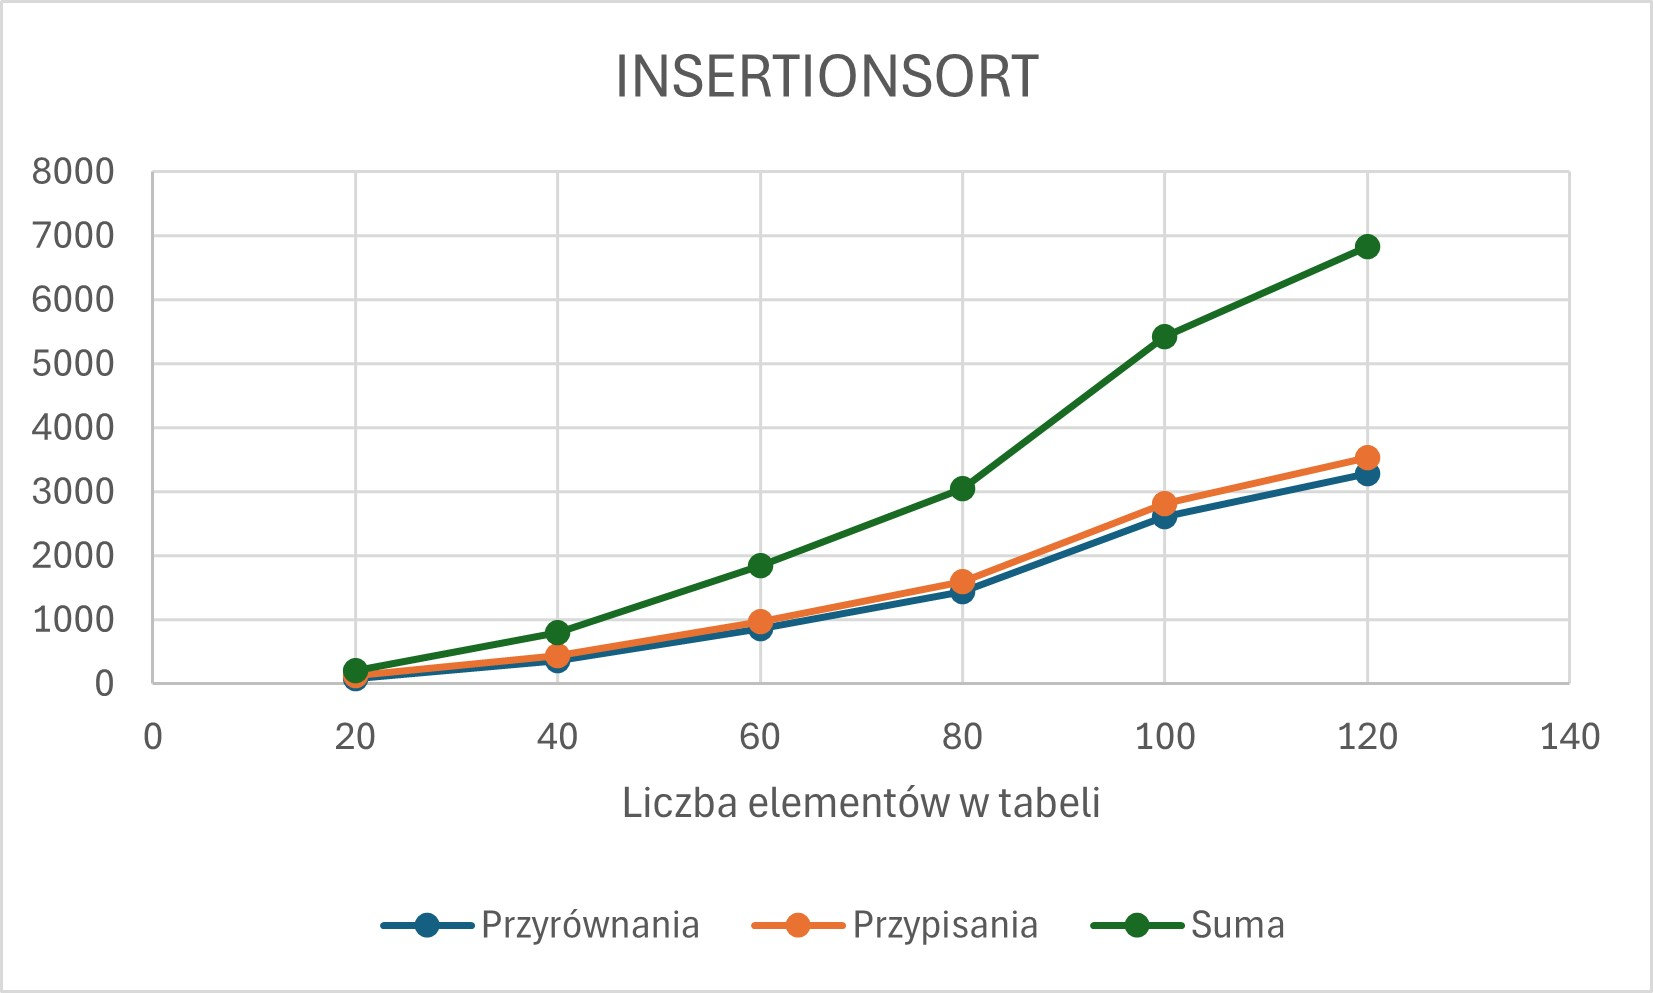
\includegraphics[width=0.9\textwidth]{INS1.jpg}
		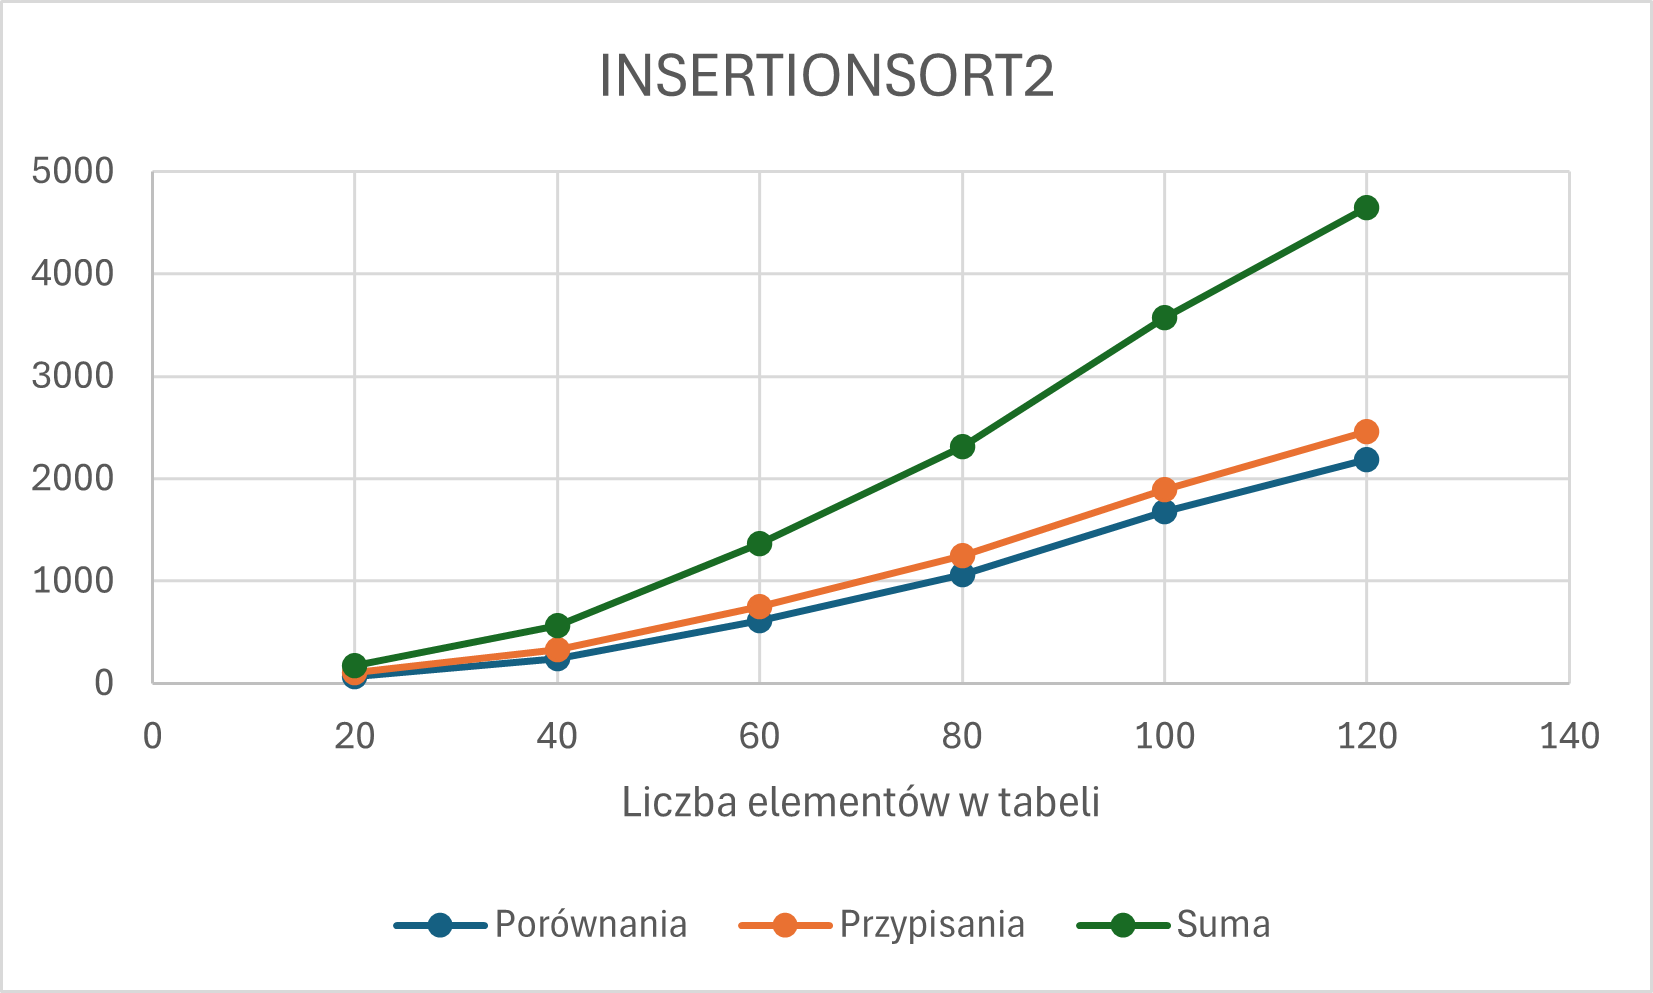
\includegraphics[width=0.9\textwidth]{INS2.png}
	\end{figure}
	
	Oba algorytmy są odmianami algorytmu sortowania przez wstawianie, które ma złożoność czasową \( O(n^2) \) INSERTIONSORT wykonuje operacje na każdym elemencie po kolei, natomiast INSERTIONSORT2 optymalizuje sortowanie, operując na dwóch elementach naraz. Na obu wykresach widzimy, że liczba porównań i przypisań rośnie wykładniczo w stosunku do liczby elementów w tabeli. Oznacza to, że przy większych rozmiarach tablic oba algorytmy stają się coraz bardziej kosztowne obliczeniowo. Widać, że INSERTIONSORT2 ma lekko mniejszą liczbę porównań i przypisań niż INSERTIONSORT.
	
	\newpage
	\section*{Zadanie 2}
	\begin{lstlisting}[language=C++, tabsize=3]
	void MERGE(int A[], int p, int q, int r) {
		int n1 = q - p + 1;
		int n2 = r - q;
		
		int L[n1 + 1];
		int R[n2 + 1];
		
		for (int i = 0; i < n1; i++)
		L[i] = A[p + i];
		for (int j = 0; j < n2; j++)
		R[j] = A[q + 1 + j];
	\end{lstlisting}
	Tworzone są dwie nowe tablice: L[] i R[], które przechowują elementy z dwóch podtablic z tablicy A[]. Do tablicy L[] kopiowane są elementy z zakresu od A[p] do A[q], a do tablicy R[] elementy z zakresu od A[q+1] do A[r].
	\begin{lstlisting}[language=C++, tabsize=3]
	for (int k = p; k <= r; k++) {
		if (L[i] <= R[j]) {
			A[k] = L[i];
			i++;
		} else {
			A[k] = R[j];
			j++;
		}
	\end{lstlisting}
	Następnie elementy z L[] i R[] są porównywane i z powrotem umieszczane w tablicy A[] w taki sposób, że wynikowa tablica pozostaje posortowana.
	\begin{lstlisting}[language=C++, tabsize=3]
	void MERGESORT(int A[], int p, int r) {
		if (p < r) {
			int q = (p + r) / 2;
			MERGESORT(A, p, q);
			MERGESORT(A, q + 1, r);
			MERGE(A, p, q, r);
		}
	}
	\end{lstlisting}
	Funkcja sprawdza, czy przedział ma więcej niż jeden element. Jeśli tak, to dzieli tablicę na dwie mniejsze podtablice. Następnie wywołuje rekurencyjnie MERGESORT dla lewej i prawej części tablicy. Po posortowaniu obu części, wywoływana jest funkcja MERGE, która scala te części w jedną posortowaną podtablicę.
	\begin{lstlisting}[language=C++, tabsize=3]
	void MERGE2(int A[], int p, int q1, int q2, int r) {
		int n1 = q1 - p + 1;
		int n2 = q2 - q1;
		int n3 = r - q2;
		
		int L[n1 + 1], M[n2 + 1], R[n3 + 1];
		
		for (int i = 0; i < n1; i++)
		L[i] = A[p + i];
		
		for (int j = 0; j < n2; j++)
		M[j] = A[q1 + 1 + j];
		
		for (int k = 0; k < n3; k++)
		R[k] = A[q2 + 1 + k];
	\end{lstlisting}
	Zamiast dwóch podtablic, w funkcji MERGE2 mamy trzy podtablice. Podobnie jak w poprzednim przykładzie, wartości z tych podtablic są porównywane, a następnie scala się je w jedną posortowaną tablicę.
	\begin{lstlisting}[language=C++, tabsize=3]
	void MERGESORT2(int A[], int p, int r) {
		if (p < r) {
			porownania++;
			int q1 = p + (r - p) / 3;
			int q2 = p + 2 * (r - p) / 3;
			
			MERGESORT2(A, p, q1);
			MERGESORT2(A, q1 + 1, q2);
			MERGESORT(A, q2 + 1, r);
			
			MERGE2(A, p, q1, q2, r);
		}
	}
	\end{lstlisting}
	Zamiast dzielić tablicę na dwie połowy, funkcja MERGESORT2 dzieli tablicę na trzy części. Rekurencyjnie wywoływane są trzy MERGESORT2 na trzech mniejszych podtablicach.
	
	\begin{figure}[H]
		\centering
		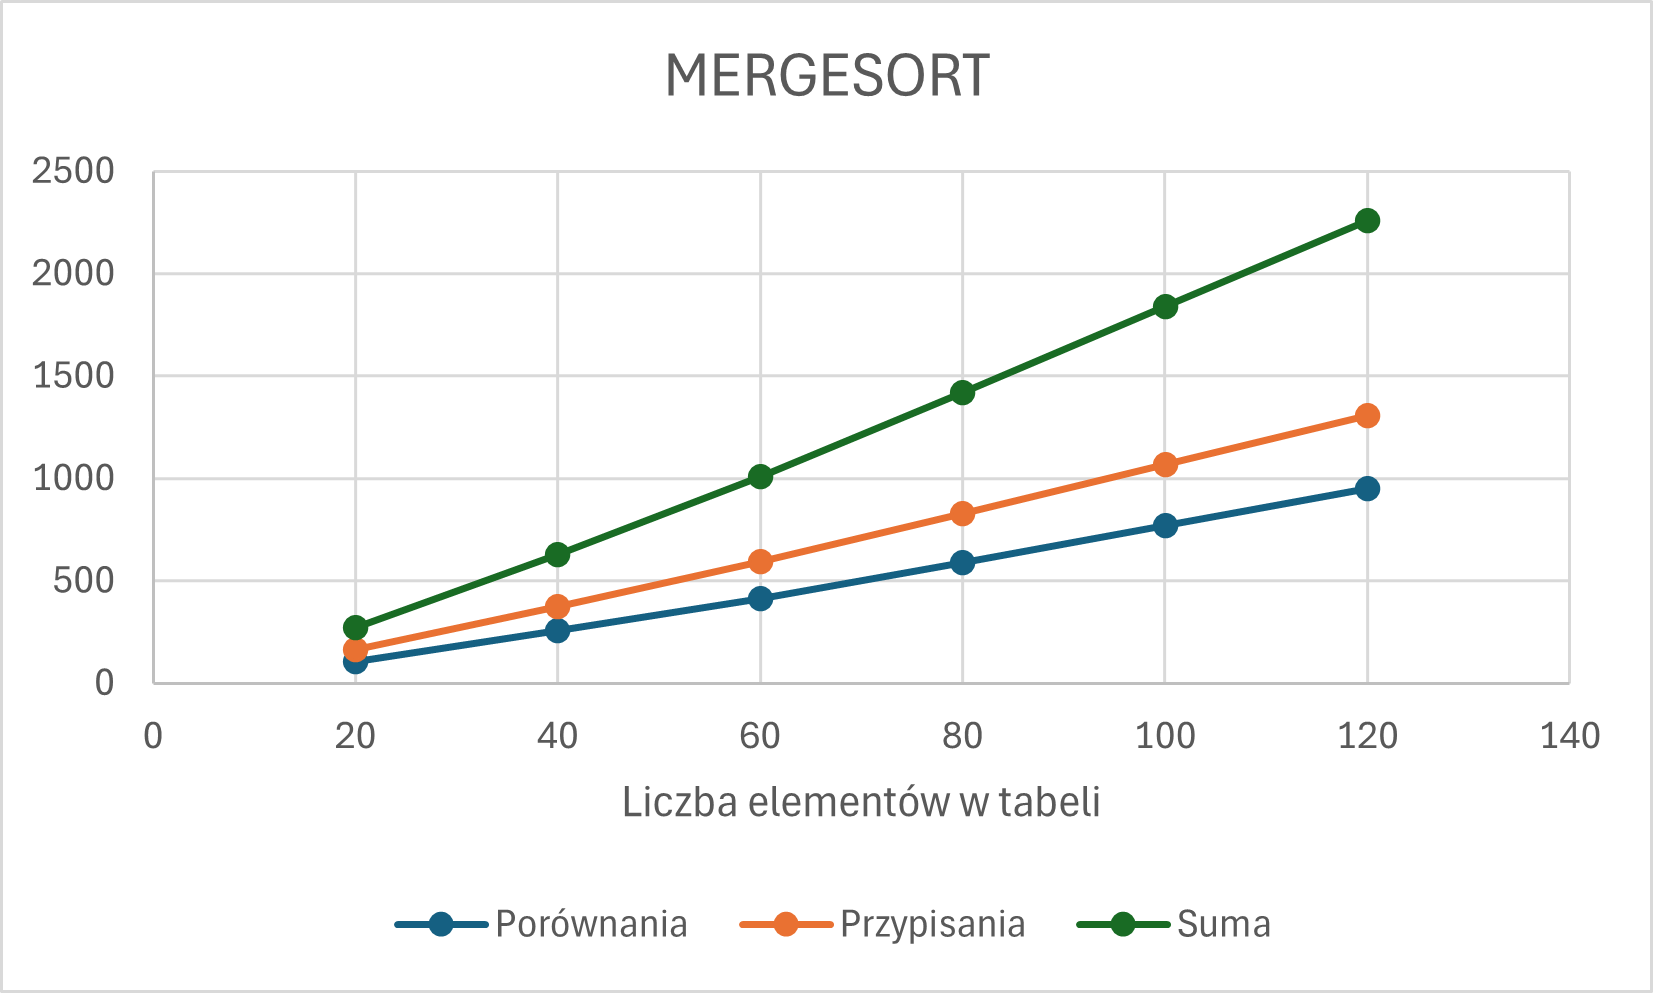
\includegraphics[width=0.9\textwidth]{MER1.png}
		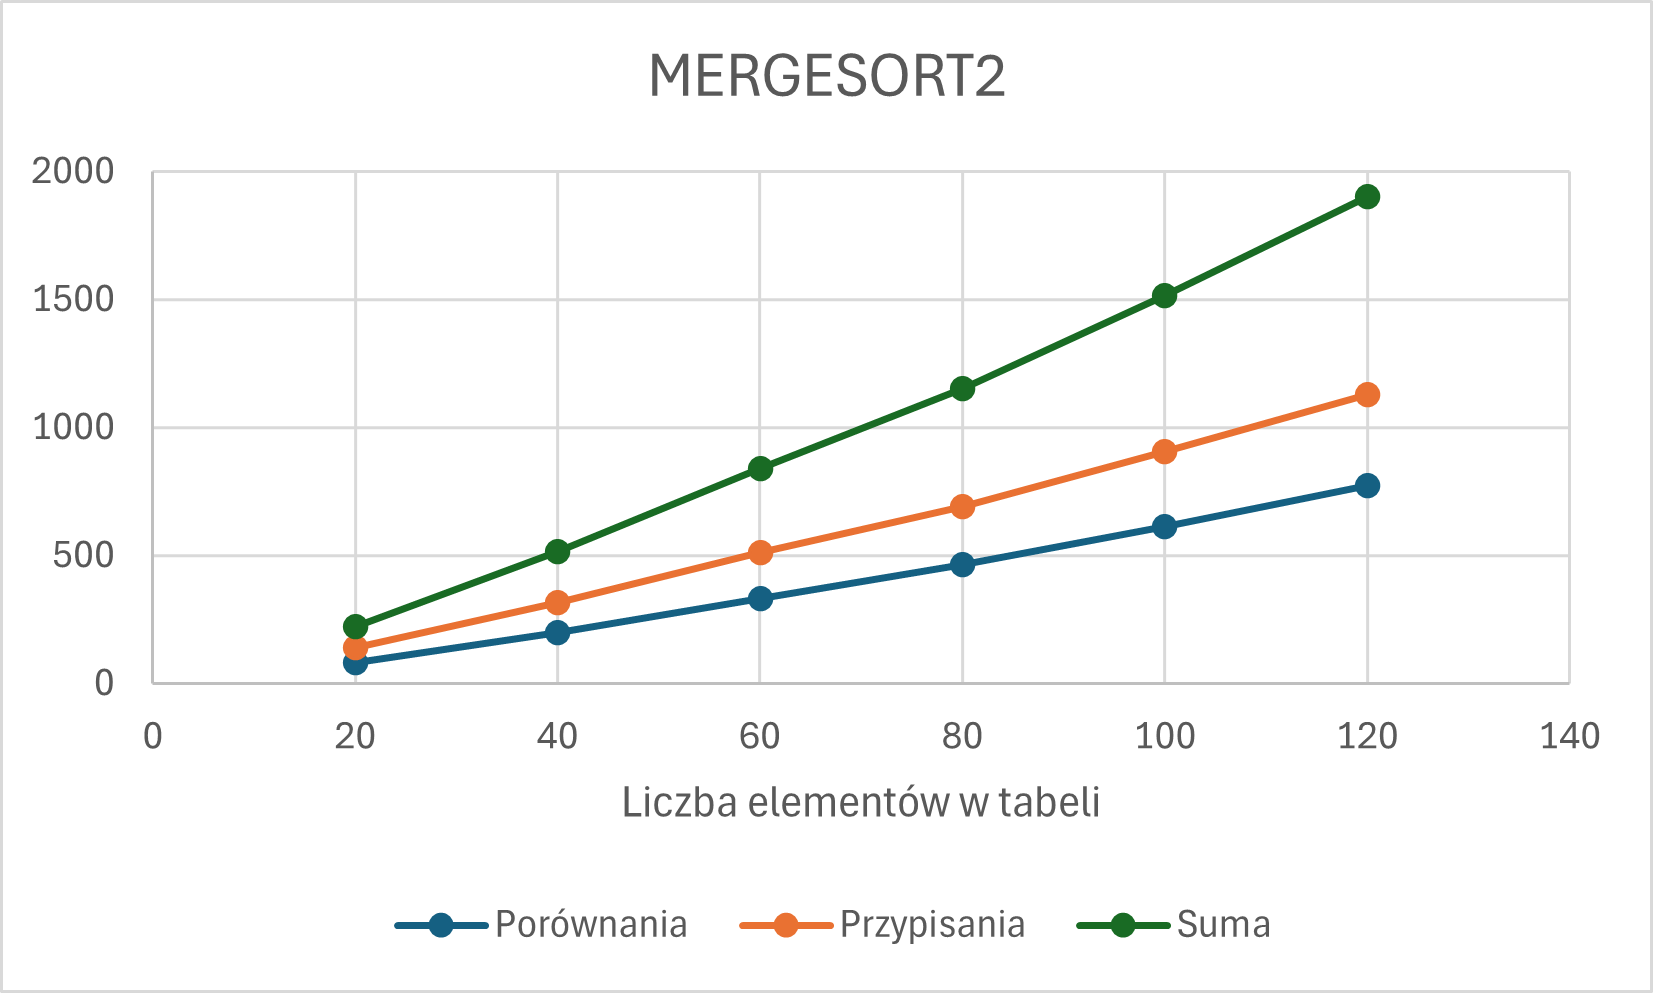
\includegraphics[width=0.9\textwidth]{MER2.png}
	\end{figure}
	
	
	Klasyczny Merge Sort ma złożoność czasową \(O(nlogn)\), przy czym stały współczynnik zależy od liczby porównań i przypisań. Liczba porównań i liczba przypisań rośnie liniowo w obu algorytmach, ale są one nieco niższe w MERGESORT2 niż MERGESORT.
	
	\newpage
	\section*{Zadanie 3}
	\begin{lstlisting}[language=C++, tabsize=3] 
	void HEAPIFY(int A[], int i, int n) {
		int l = LEFT(i);
		int r = RIGHT(i);
		int najwiekszy = i;
		
		if (l < n && A[l] > A[i]) {
			najwiekszy = l;
		}
		
		if (r < n && A[r] > A[najwiekszy]) {
			najwiekszy = r;
		}
		
		if (najwiekszy != i) {
			swap(A[i], A[najwiekszy]);
			HEAPIFY(A, najwiekszy, n);
		}
	}
	\end{lstlisting}
Funkcja HEAPIFY dba o to, by węzeł \(i\) w kopcu był większy od swoich dzieci (LEFT(i) i RIGHT(i)). Jeśli któreś dziecko jest większe, zamienia je miejscami z \(i\) i wywołuje się ponownie dla tego dziecka, aż cała struktura będzie poprawna.\\

Następnie funkcja BUILD\_HEAP tworzy kopiec maksymalny z nieposortowanej tablicy A[] o rozmiarze \(n\).
	\begin{lstlisting}[language=C++, tabsize=3] 
	void HEAPSORT(int A[], int n) {
		BUILD_HEAP(A, n);
		
		for (int i = n - 1; i >= 1; i--) {
			swap(A[0], A[i]);	
			n--;
			HEAPIFY(A, 0, n);
		}
	}
	\end{lstlisting}
	Najpierw funkcja buduje kopiec maksymalny (BUILD\_HEAP), a następnie iteracyjnie zamienia największy element z ostatnim elementem tablicy. Po każdej zamianie, zmniejsza rozmiar kopca (czyli \(n\)) i wywołuje HEAPIFY, aby przywrócić właściwość kopca dla pozostałych elementów.
	\begin{lstlisting}[language=C++, tabsize=3] 
	void HEAPIFY2(int A[], int i, int n) {
		int l = LEWY2(i);
		int s = SRODKOWY2(i);
		int p = PRAWY2(i);
		int najwiekszy = i;
		
		if (l < n && A[l] > A[i]) {
			najwiekszy = l;
		}
		
		if (s < n && A[s] > A[najwiekszy]) {
			najwiekszy = s;
		}
		
		if (p < n && A[p] > A[najwiekszy]) {
			najwiekszy = p;
		}
		
		if (najwiekszy != i) {
			swap(A[i], A[najwiekszy]);
			HEAPIFY2(A, najwiekszy, n);
		}
	}
	\end{lstlisting}
	Zamiast porównywać węzeł z dwoma dziećmi, teraz porównuje z trzema dziećmi (lewe, środkowe i prawe). Działa na drzewie trójkowym, gdzie dla każdego węzła sprawdzane są trzy potencjalne potomki, i zamienia węzeł z największym, jeśli któryś z potomków ma większą wartość.
	\begin{lstlisting}[language=C++, tabsize=3] 
	
	void HEAPSORT2(int A[], int n) {
		BUILD_HEAP2(A, n);
		for (int i = n - 1; i >= 1; i--) {
			swap(A[0], A[i]);
			n--;
			HEAPIFY2(A, 0, n);
		}
	}
	\end{lstlisting}
	Funkcja HEAPSORT2 jest podobna do poprzedniej wersji, ale działa na drzewie trójkowym, więc wykorzystuje odpowiednie funkcje (HEAPIFY2 i BUILD\_HEAP2).
	
	\begin{figure}[H]
		\centering
		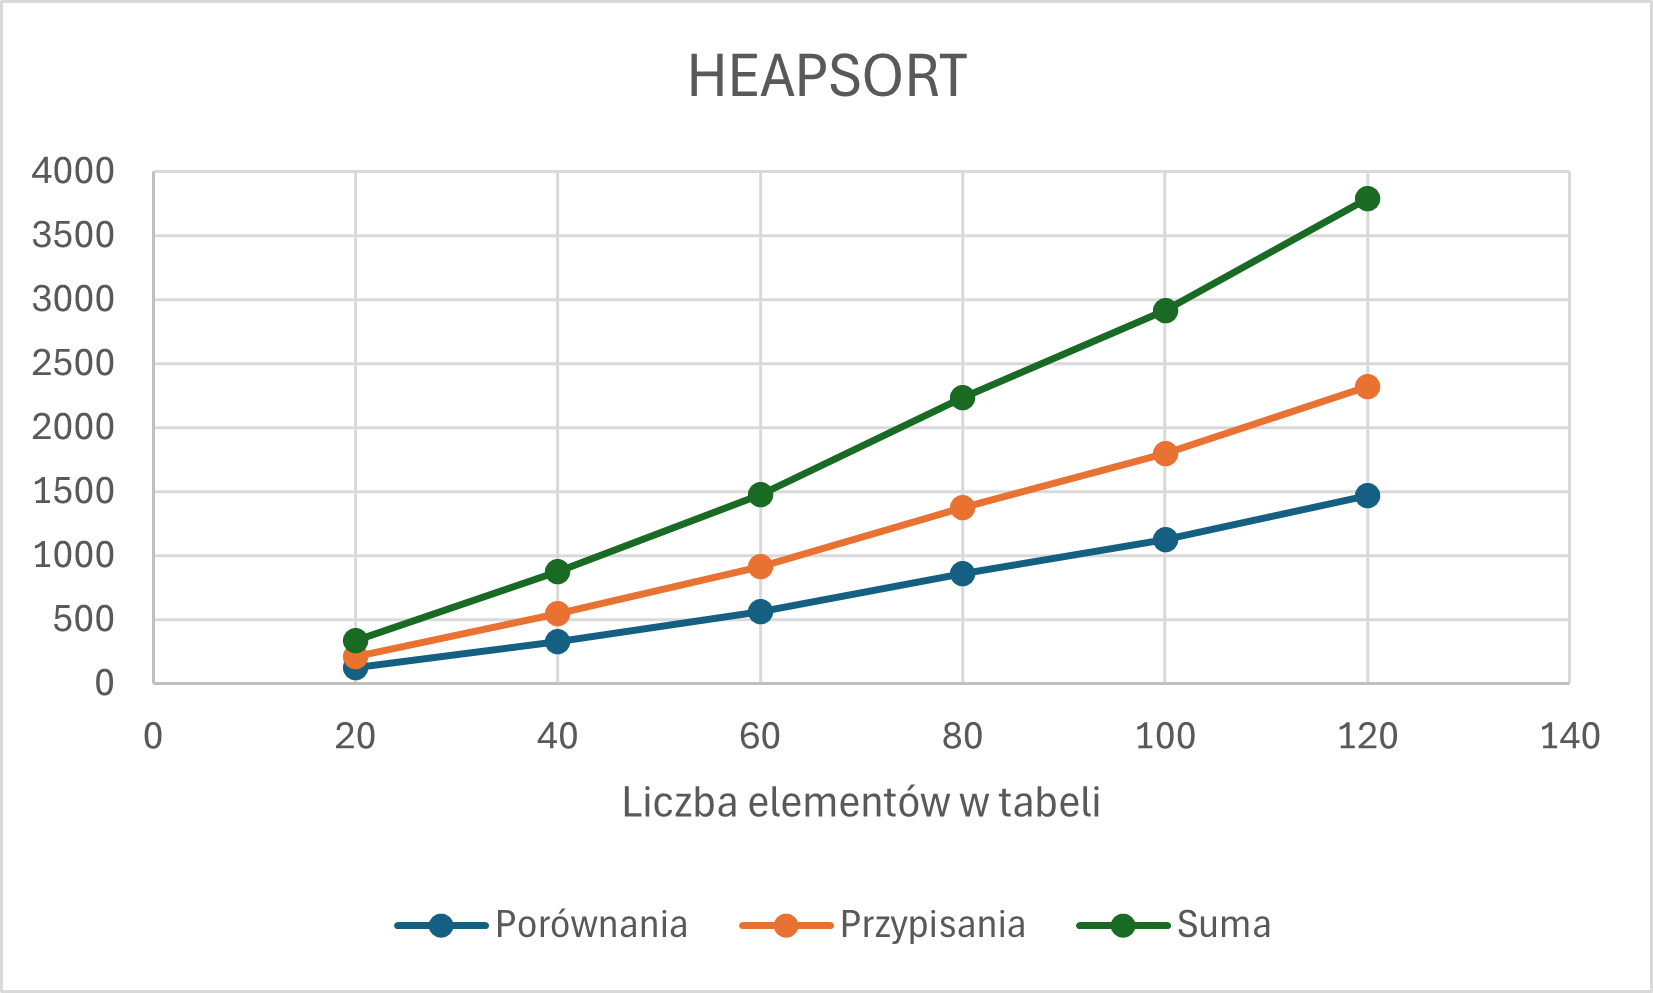
\includegraphics[width=0.9\textwidth]{HEAP1.png}
		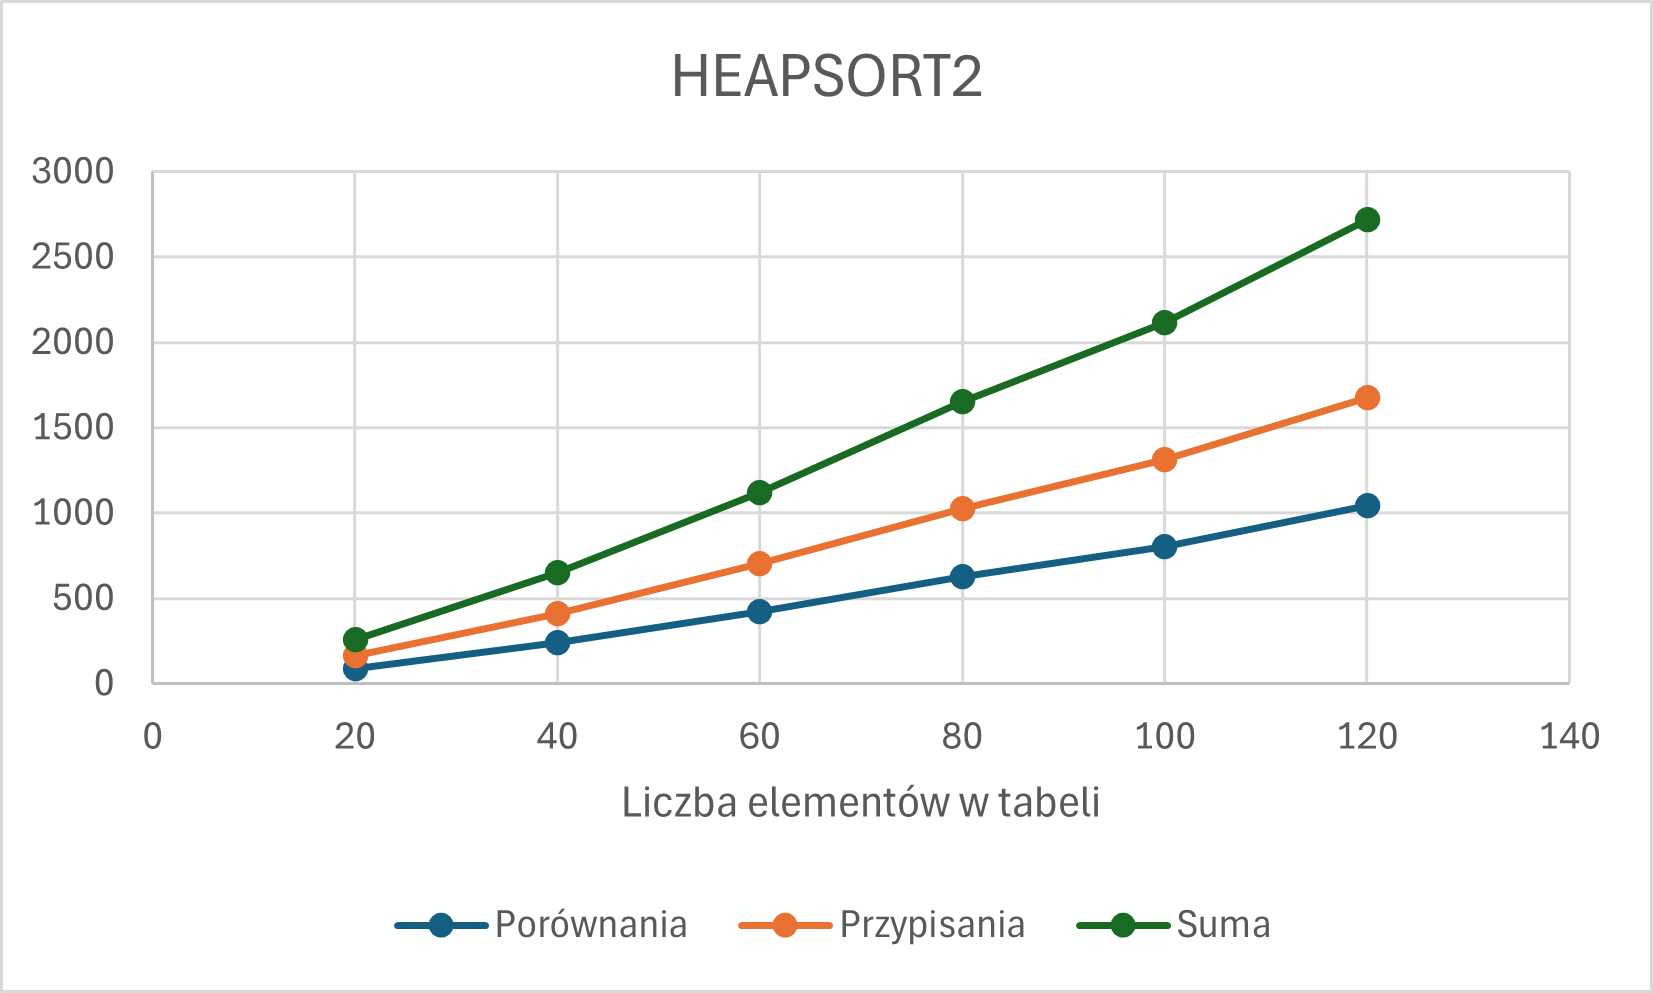
\includegraphics[width=0.9\textwidth]{HEAP2.png}
	\end{figure}
	
	
	Złożoność czasowa algorytmu wynosi \(O(nlogn)\) i wpływa na nią liczba elementów do posortowania. Z wykresów widać że w obu funkcjach liczba przypisań i liczba porównań rośnie wraz z ilością elementów. Liczby te są nieco niższe dla HEAPSORT2. 
	
	\newpage
	\section*{Wszystkie funkcje}
	\begin{figure}[H]
		\centering
		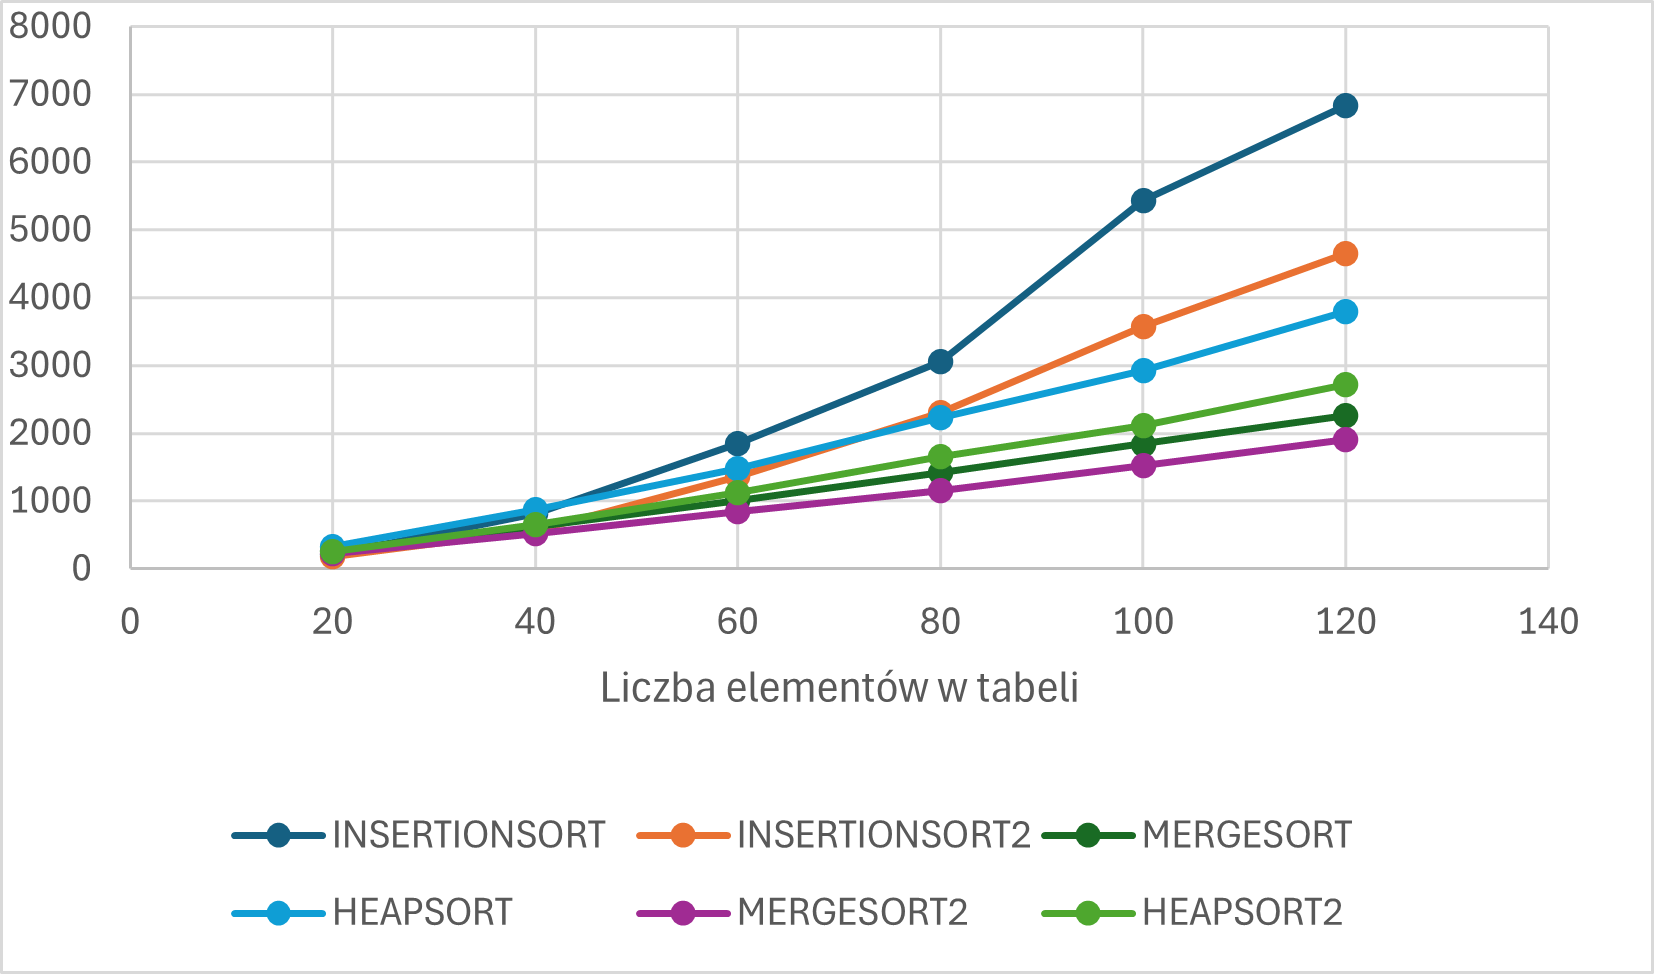
\includegraphics[width=0.9\textwidth]{Wszystko.png}
	\end{figure}
	
	INSERTIONSORT2 jest bardziej zoptymalizowaną funkcją niż INSERTIONSORT. Te algorytmy działą dobrze dla małych zbiorów danych, ale jego wydajność szybko spada w przypadku większych. Algorytmy MERGESORT i MERGESORT2 różnią się, ale oba wykazują stosunkowo wolniejszy wzrost liczby operacji w porównaniu do INSERTIONSORT. MERGESORT2 wydaje się być nieco bardziej optymalny niż MERGESORT. Algorytmy sortowania takie jak MERGESORT i HEAPSORT lepiej sprawdzają się w przypadku dużych tablic, ponieważ ich wzrost liczby operacji jest znacznie wolniejszy niż w przypadku algorytmu INSERTIONSORT. A optymalizacje w implementacjach (jak w MERGESORT2 i HEAPSORT2) mogą prowadzić do zauważalnych różnic w liczbie operacji, zwłaszcza przy większych zbiorach danych.
\end{document}